\documentclass[presentation]{beamer}

\usepackage{tikz}
\usetikzlibrary{trees,calc,positioning}
\usetikzlibrary{shapes, shapes.geometric}
% https://tex.stackexchange.com/questions/27171/padded-boundary-of-convex-hull
\newcommand{\convexpath}[2]{
  [
  create hullcoords/.code={
    \global\edef\namelist{#1}
    \foreach [count=\counter] \nodename in \namelist {
      \global\edef\numberofnodes{\counter}
      \coordinate (hullcoord\counter) at (\nodename);
    }
    \coordinate (hullcoord0) at (hullcoord\numberofnodes);
    \pgfmathtruncatemacro\lastnumber{\numberofnodes+1}
    \coordinate (hullcoord\lastnumber) at (hullcoord1);
  },
  create hullcoords
  ]
  ($(hullcoord1)!#2!-90:(hullcoord0)$)
  \foreach [
  evaluate=\currentnode as \previousnode using \currentnode-1,
  evaluate=\currentnode as \nextnode using \currentnode+1
  ] \currentnode in {1,...,\numberofnodes} {
    let \p1 = ($(hullcoord\currentnode) - (hullcoord\previousnode)$),
    \n1 = {atan2(\y1,\x1) + 90},
    \p2 = ($(hullcoord\nextnode) - (hullcoord\currentnode)$),
    \n2 = {atan2(\y2,\x2) + 90},
    \n{delta} = {Mod(\n2-\n1,360) - 360}
    in
    {arc [start angle=\n1, delta angle=\n{delta}, radius=#2]}
    -- ($(hullcoord\nextnode)!#2!-90:(hullcoord\currentnode)$)
  }
}
\usepackage{booktabs}
\usepackage{pgf}
\usepackage{pgfplots}
\pgfplotsset{compat=1.13}
\usepackage{pgfplotstable}
\usepackage{appendixnumberbeamer}
\usepackage{amsmath}
\usepackage{pifont}
\newcommand{\cmark}{\ding{51}}
\newcommand{\xmark}{\ding{55}}
\DeclareMathOperator{\grad}{grad}
\DeclareMathOperator{\tr}{tr}
\let\div\relax
\DeclareMathOperator{\div}{div}
\DeclareMathOperator{\curl}{curl}
\date{18th September 2018}
\usetheme{metropolis}
\metroset{progressbar=frametitle}

\usepackage{algpseudocode}
\renewcommand{\vec}[1]{\ensuremath{\boldsymbol{#1}}}
\newcommand{\ddt}[1]{\frac{\partial #1}{\partial t}}
\newcommand{\zhat}{\hat{\vec{z}}}
\newcommand{\W}{\ensuremath{\mathbb{W}}}

\newcommand{\inner}[1]{\left\langle #1 \right \rangle}

\newcommand{\KSP}[2]{\ensuremath{\mathcal{K}\left(#1, \mathbb{#2}\right)}}
\newcommand{\ksp}[1]{\KSP{#1}{#1}}

\newcommand{\highlight}[1]{\colorbox{red!20}{\color{black} #1}}
\newcommand{\arxivlink}[2]{%
  \href{http://www.arxiv.org/abs/#1}%
  {\texttt{arXiv:\,#1\,[#2]}}%
}
\newcommand{\doilink}[1]{%
  \href{http://dx.doi.org/#1}%
  {\texttt{doi:\,#1}{}}%
}

\author{Lawrence Mitchell\inst{1,*} \\ {\scriptsize C.J.~Cotter,
    P.E.~Farrell, D.A.~Ham, M.~Homolya, P.H.J.~Kelly, R.C.~Kirby, F.~Wechsung \ldots}}
\institute{
\inst{1}Department of Computer Science, Durham University

\inst{*}\texttt{lawrence.mitchell@durham.ac.uk}
}

\graphicspath{{./\jobname.figures/}{../pictures/}}

\usepackage[url=false,
doi=true,
isbn=false,
style=authoryear,
maxnames=5,
giveninits=true,
uniquename=init,
backend=biber]{biblatex}

\usepackage{xspace}
\let\Re\relax
\DeclareMathOperator{\Re}{Re}
\newcommand{\honev}{\ensuremath{{H}^1(\Omega; \mathbb{R}^d)}\xspace}
\newcommand{\ltwov}{\ensuremath{{L}^2(\Omega; \mathbb{R}^d)}\xspace}
\newcommand{\ltwo}{\ensuremath{{L}^2(\Omega)}\xspace}
\newcommand{\laplace}{\ensuremath{\Delta}\,}
\newcommand{\rt}{\ensuremath{\mathrm{RT}_0}\xspace}
\newcommand{\nd}{\ensuremath{\mathrm{ND}_0}\xspace}
% \let\ker\relax
% \DeclareMathOperator{\ker}{ker}
\newcommand{\kerdiv}{\ker\div}
\newcommand{\kercurl}{\ker\curl}
\newcommand{\eker}{\ensuremath{e^{\ker}}\xspace}
\newcommand{\ds}{\ \text{d}s}
\newcommand{\dx}{\ \text{d}x}
\newcommand{\Pq}{\ensuremath{\mathrm{P}_{Q_h}}}
\newcommand{\PqK}{\ensuremath{\mathrm{P}_{Q_h(K)}}}
\newcommand{\Ptwo}{\ensuremath{\mathbb{P}_2}\xspace}
\newcommand{\Pthree}{\ensuremath{\mathbb{P}_3}\xspace}
\newcommand{\PtwoPzero}{\ensuremath{[\mathbb{P}_2]^2\mathrm{-}\mathbb{P}_0}\xspace}
\newcommand{\PtwothreePzero}{\ensuremath{[\mathbb{P}_2]^3\mathrm{-}\mathbb{P}_0}\xspace}
\newcommand{\PthreePzero}{\ensuremath{[\mathbb{P}_3]^3\mathrm{-}\mathbb{P}_0}\xspace}
\newcommand{\Pzero}{\ensuremath{\mathbb{P}_0}\xspace}
\newcommand{\Pv}{\ensuremath{\mathbb{P}_v}\xspace}
\newcommand{\BR}{\ensuremath{\left[\mathbb{P}_1 \oplus B^F_3\right]}\xspace}
\newcommand{\PoneFB}{\ensuremath{\mathbb{P}_1 \oplus B^F_3}\xspace}
\newcommand{\PtwoFB}{\ensuremath{\mathbb{P}_2 \oplus B^F_3}\xspace}
\newcommand{\BRzero}{\ensuremath{\BR^3\mathrm{-}\mathbb{P}_0}\xspace}
\newcommand{\fmw}{\ensuremath{\left(\mathbb{P}_2 \oplus B^F_3\right)}\xspace}
\newcommand{\fmwzero}{\ensuremath{\fmw^3\mathrm{-}\mathbb{P}_0}\xspace}
%\newcommand{\advect}[2]{\ensuremath{(\nabla #1) \cdot #2}}
\newcommand{\advect}[2]{\ensuremath{(#2 \cdot \nabla) #1}}
\newcommand{\mesh}{\ensuremath{\mathcal{M}}\xspace}
\newcommand{\Ac}{\ensuremath{\mathcal{A}}}
\newcommand{\Bc}{\ensuremath{\mathcal{B}}}
\setbeamertemplate{bibliography item}{}

\renewcommand{\bibfont}{\fontsize{7}{7}\selectfont}
\addbibresource{references.bib}

\setlength{\bibitemsep}{1ex}
\setlength{\fboxsep}{1pt}

\renewbibmacro{in:}{}
\DeclareFieldFormat[article]{volume}{\textbf{#1}}
\DeclareFieldFormat{doi}{%
  doi\addcolon%
  {\scriptsize\ifhyperref{\href{http://dx.doi.org/#1}{\nolinkurl{#1}}}
    {\nolinkurl{#1}}}}
\AtEveryBibitem{%
\clearfield{pages}%
\clearfield{issue}%
\clearfield{number}%
}

\usepackage{minted}
\RecustomVerbatimEnvironment{Verbatim}{BVerbatim}{}


\title{From symbolic mathematics to fast solvers for finite element problems}

\begin{document}

\maketitle

% \begin{abstract}
%   One of the great and enduring successes of numerical computing is
%   the capturing of mathematical abstractions in software.  This allows
%   the programmer to express the intent of their code, without
%   specifying its low-level implementation.  We then automate the
%   synthesis of efficient code by using (or writing) compilers.

%   In the context of solving numerical PDEs, the finite element method
%   is particularly amenable to this approach.  For many problems, the
%   choice of discretisation completely specifies the mathematical
%   intent.  A symbolic description of the PDE can then be manipulated
%   by a domain-specific compiler to produce a high-performance
%   implementation.

%   In this talk, I will present a concrete realisation of these ideas,
%   embodied in the finite element software Firedrake
%   (www.firedrakeproject.org).  I will discuss how capturing and
%   exploiting symbolic structure in numerical software greatly
%   simplifies model development, while simultaneously permitting the
%   synthesis of a high performance implementation.

%   I will then discuss recent work extending these same ideas to the
%   development of preconditioners, illustrating with some recent work
%   on scalable solvers for the three-dimensional stationary
%   Navier-Stokes equations.
% \end{abstract}

% People:
% Jerome Droniou
% Michael Page
% Hans de Sterck
% Philip Hall
% Steve Siems
% Yann Bernard
% Simon Clarke
% Julie Clutterbuck
% Anja Slim
% Kengo Deguchi
% Christian Thomas

\begin{frame}
  \frametitle{Outline}

  \begin{itemize}
  \item Automated finite elements
    \begin{itemize}
    \item Fast implementations thereof
    \end{itemize}
  \item Multilevel solvers for coupled problems
    \begin{itemize}
    \item Stationary Navier-Stokes
    \end{itemize}
  \item Future directions
  \end{itemize}
\end{frame}

\begin{frame}[fragile]
  \frametitle{Code that looks like maths}
  \begin{columns}
    \begin{column}{0.47\framewidth}
      {\footnotesize
        Find $(u, p, T) \in V\times W\times Q$ s.t.
        \begin{align*}
          \int\!\nabla u \cdot \nabla v + (u \cdot \nabla u) \cdot v \\
          - p\nabla\cdot v + \frac{\text{Ra}}{\text{Pr}} Tg \hat{z} \cdot v\,\text{d}x &= 0 \\
          \int\!\nabla\cdot u q\,\text{d}x&= 0\\
          \int\! (u\cdot \nabla T) S + \text{Pr}^{-1} \nabla T \cdot \nabla
          S\,\text{d}x &= 0\\
          \quad \forall\, (v,q,T) \in V\times W \times Q
        \end{align*}
        }
    \end{column}
      \begin{column}{0.52\framewidth}
\begin{minted}[fontsize=\tiny]{python}
from firedrake import *
mesh = Mesh(...)
V = VectorFunctionSpace(mesh, "CG", 2)
W = FunctionSpace(mesh, "CG", 1)
Q = FunctionSpace(mesh, "CG", 1)
Z = V * W * Q
Ra = Constant(...)
Pr = Constant(...)
upT = Function(Z)
u, p, T = split(upT)
v, q, S = TestFunctions(Z)
bcs = [...]

F = (inner(grad(u), grad(v))
     + inner(dot(grad(u), u), v)
     - inner(p, div(v))
     + (Ra/Pr)*inner(T*g, v)
     + inner(div(u), q)
     + inner(dot(grad(T), u), S)
     + (1/Pr) * inner(grad(T), grad(S)))*dx

solve(F == 0, upT, bcs=bcs)
\end{minted}
      \end{column}
  \end{columns}
\end{frame}

\begin{frame}
  \frametitle{Finite elements I}
  \begin{align*}
    F(u) = 0 \text{ in $\Omega$}\\
    \text{+ boundary conditions}
  \end{align*}
  Seek weak solution in some space of functions $V(\Omega)$.

  Now we need to solve the (infinite dimensional) problem, find $u\in V$ s.t.
  \begin{equation*}
    \int_\Omega \!F(u) v\, \text{d}x = 0 \quad \forall\, v \in V
  \end{equation*}
  Choose finite dimensional subspace $V_h \subset V$, find $u_h \in V_h$ s.t.
  \begin{equation*}
    \int_\Omega \!F(u_h) v_h\, \text{d}x = 0 \quad \forall\, v_h \in V_h
  \end{equation*}
\end{frame}
\begin{frame}
  \frametitle{Finite elements II}
  \begin{overlayarea}{\textwidth}{0.5\textheight}
    \only<1>{Divide domain $\Omega$\dots
    \begin{center}
      \begin{tikzpicture}
        \draw[very thick, line cap=rect] (0,0) -- (5, 0) (0, 0) arc
        (180:360:2.5);
      \end{tikzpicture}
    \end{center}}
  \only<2>{\dots{}into triangulation $\mathcal{T}$\dots
    \begin{center}
        \begin{tikzpicture}
          \path (0,0) arc[radius=2.5, start angle=180, end angle=360]
          node[name=E,pos=0,swap] {} node[name=F,pos=0.25,swap] {}
          node[name=G,pos=0.5,swap] {} node[name=H,pos=0.82,swap] {}
          node[name=I,pos=1,swap] {};
          \node (A) at (2.5, 0) {};
          \node (B) at (1.4, -0.7) {};
          \node (C) at (3.4, -1.2) {};
          \node (D) at (1.8, -1.5) {};

          \draw[color=black, very thick, line cap=butt, line
          join=round] (E.center) -- (A.center) -- (I.center) --
          (H.center) -- (G.center) -- (F.center) -- (E.center) --
          cycle; \draw[color=black, very thick, line cap=butt, line
          join=round] (E.center) -- (B.center) -- (D.center) --
          (F.center) -- (B.center); \draw[color=black, very thick,
          line cap=butt, line join=round] (G.center) -- (D.center) --
          (C.center) -- (G.center); \draw[color=black, very thick,
          line cap=butt, line join=round] (B.center) -- (A.center) --
          (C.center) -- (B.center); \draw[color=black, very thick,
          line cap=butt, line join=round] (H.center) -- (C.center) --
          (I.center);
        \end{tikzpicture}
    \end{center}
  }
  \only<3>{\dots{}and choose basis with finite support.
    \begin{center}
        \begin{tikzpicture}
          \path (0,0) arc[radius=2.5, start angle=180, end angle=360]
          node[name=E,pos=0,swap] {} node[name=F,pos=0.25,swap] {}
          node[name=G,pos=0.5,swap] {} node[name=H,pos=0.82,swap] {}
          node[name=I,pos=1,swap] {}; \node (A) at (2.5, 0) {}; \node
          (B) at (1.4, -0.7) {}; \node (C) at (3.4, -1.2) {}; \node
          (D) at (1.8, -1.5) {};

        \path[fill=gray!50] (E.center) -- (A.center) -- (B.center) --
        (F.center) --cycle;
          \draw[color=black, very thick, line cap=butt, line
          join=round] (E.center) -- (A.center) -- (I.center) --
          (H.center) -- (G.center) -- (F.center) -- (E.center) --
          cycle; \draw[color=black, very thick, line cap=butt, line
          join=round] (E.center) -- (B.center) -- (D.center) --
          (F.center) -- (B.center); \draw[color=black, very thick,
          line cap=butt, line join=round] (G.center) -- (D.center) --
          (C.center) -- (G.center); \draw[color=black, very thick,
          line cap=butt, line join=round] (B.center) -- (A.center) --
          (C.center) -- (B.center); \draw[color=black, very thick,
          line cap=butt, line join=round] (H.center) -- (C.center) --
          (I.center);
        \end{tikzpicture}
      \end{center}
      }
  \end{overlayarea}
\end{frame}

\begin{frame}
  \frametitle{Finite elements III}
  Integrals become sum over element integrals
  \begin{equation*}
    \int_\Omega\! F(u_h) v_h \, \text{d}x =
    \sum_{e \in \mathcal{T}} \int_e\! F(u_h)v_h\, \text{d}x
  \end{equation*}

  (Usually) perform element integrals with numerical quadrature
  \begin{equation*}
    \int_e F(u_h)v_h\,\text{d}x = \sum_q w_q F(u_h(q)) v_h(q)\,\text{d}x
  \end{equation*}

  Replace $u_h(q), v_h(q)$ with expansion in finite element basis
  \begin{align*}
    u_h(q) &= \sum_i u_h^i \phi_i(q)\\
    v_h(q) &= \phi_j(q)\\
  \end{align*}
\end{frame}

\begin{frame}
  \frametitle{Looking for abstractions}
  \begin{itemize}
  \item Mathematics just says ``here is the integral to compute on each
    element, do that everywhere''
  \item Computer implementation chooses how to do so
  \end{itemize}
  \begin{block}{Assertion(s)}
    Having chosen a discretisation, writing the element integral is ``mechanical''.

    With an element integral in hand, integrating over a mesh is
    ``mechanical''.
  \end{block}

  \begin{corollary}
    Computers are good at mechanical things, why don't we get the
    computer to write them for us?
  \end{corollary}
\end{frame}

\begin{frame}
  \frametitle{Firedrake \url{www.firedrakeproject.org}}

  \begin{columns}
    \begin{column}{0.8\textwidth}
      \begin{quote}
        {\normalfont [\ldots]} an automated system for the solution of
        partial differential equations using the finite element
        method.
      \end{quote}
    \end{column}
    \begin{column}{0.2\textwidth}
      
\includegraphics[width=0.8\textwidth]{firedrake-small}
    \end{column}
  \end{columns}
  \begin{overlayarea}{\textwidth}{0.8\textheight}
    \begin{onlyenv}<1>
      \begin{itemize}
      \item Written in Python.
      \item Finite element problems specified with \emph{embedded}
        domain specific language, UFL \parencite{Alnaes:2014} from the
        FEniCS project.
      \item \emph{Runtime} compilation to optimised, low-level (C)
        code.
      \item PETSc for meshes and (algebraic) solvers.
      \end{itemize}

    \begin{flushright}
      {\scriptsize F.~Rathgeber, D.A.~Ham, \textbf{LM}, M.~Lange,
        F.~Luporini, A.T.T.~McRae, G.-T.~Bercea, G.R.~Markall,
        P.H.J.~Kelly. ACM Transactions on Mathematical Software,
        2016. \arxivlink{1501.01809}{cs.MS}\nocite{Rathgeber:2016}}
    \end{flushright}
  \end{onlyenv}
  \begin{onlyenv}<2>
    \begin{block}{User groups at}
      Imperial, Oxford, Bath, Leeds, Durham, Kiel, Rice, Houston,
      Exeter, Buffalo, Waterloo, Minnesota, Baylor, Texas A\&M, \dots

      Annual user \& developer meeting this year had 45 attendees.
    \end{block}
  \end{onlyenv}
\end{overlayarea}
\end{frame}


\begin{frame}[fragile]
  \frametitle{More automation}
  \begin{columns}
    \begin{column}{0.45\textwidth}
      \begin{equation*}
        a(u, v) = \int_\Omega \nabla u \cdot \nabla v\,\text{d}x \quad \forall v \in V
      \end{equation*}
\begin{minted}[fontsize=\scriptsize]{python}
V = FiniteElement("Lagrange",
                  triangle, 1)
u = TrialFunction(V)
v = TestFunction(V)
F = dot(grad(u), grad(v))*dx
\end{minted}
    \end{column}
    \hspace{0.05\textwidth}
    \begin{column}{0.45\textwidth}
      \begin{tikzpicture}
        \node[draw,rectangle, thick, text width=1in, align=center] (A)
        {\small Pen and paper};

        \node[draw, below=of A, rectangle, thick, text width=1in,
        align=center] (B) {\small High-level code};

        \node[draw, below=of B, rectangle, thick, text width=1in,
        align=center] (C) {\small Low-level code};

        \node[draw, below=of C, rectangle, thick, text width=1in,
        align=center] (D) {\small Machine code};

        \draw[-stealth] (A) -> (B) node [midway,right,text
        width=1in,align=center] {\small Manual};

        \draw[-stealth] (B) -> (C) node [midway, right, text
        width=1in, align=center]
        {\small Automated};

        \draw[-stealth] (C) -> (D) node [midway, right, text
        width=1.5in, align=center] {\small Automated (gcc)};
      \end{tikzpicture}
    \end{column}
  \end{columns}
\end{frame}

\begin{frame}[fragile]
  \frametitle{Automation enables optimisations}
  Compile UFL (symbolics) into low-level code (implementation).
  \begin{flushright}
    {\scriptsize M.~Homolya, \textbf{LM}, F.~Luporini, D.A.~Ham. SIAM
      SISC (2018). \arxivlink{1705.03667}{cs.MS}}
  \end{flushright}
  \begin{itemize}
  \item Element integral
    \begin{columns}
      \begin{column}{0.4\textwidth}
        \begin{equation*}
          \int_e \nabla u \cdot \nabla v\,\text{d}x
        \end{equation*}
      \end{column}
      \hspace{-3em}
      \begin{column}{0.6\textwidth}
\begin{minted}[fontsize=\scriptsize]{python}
V = FiniteElement("Lagrange", triangle, 1)
u = TrialFunction(V)
v = TestFunction(V)
a = dot(grad(u), grad(v))*dx
\end{minted}
      \end{column}
    \end{columns}
    \hspace{0.5\baselineskip}
  \item Is transformed to a tensor algebra expression
    {\small \begin{equation*}
        \sum_q w_q \left| d \right| \sum_{i_5} \left( \sum_{i_3}
          K_{i_3,i_5} \begin{bmatrix}
            E^{(1)}_{q,k} & E^{(2)}_{q,k}
          \end{bmatrix}_{i_3} \right)
        \left( \sum_{i_4} K_{i_4,i_5} \begin{bmatrix}
            E^{(1)}_{q,j} & E^{(2)}_{q,j}
          \end{bmatrix}_{i_4} \right)
      \end{equation*}}
  \item Multiple optimisation passes aim to minimise FLOPs required to
    evaluate this expression.
  \end{itemize}
\end{frame}

\begin{frame}
  \frametitle{Optimisation passes}
  \begin{block}{Sum factorisation}
    Spectral elements typically use \emph{tensor product} basis functions
    \begin{equation*}
      \phi_{i,q} := \phi_{(j,k),(p,r)} = \varphi_{j,p}\varphi_{k,r}
    \end{equation*}
    Tensor algebra maintains this structure, compiler exploits it for
    low-complexity evaluation of integrals.
  \end{block}
  \begin{block}{Loop transformations}
    Solve ILP problem to reorder loops, and decide how to split
    complicated expressions.
  \end{block}
  \begin{block}{Vectorisation}
    Low-level rearrangement to ease the job of C compilers in
    generating efficient code.
  \end{block}

\end{frame}

\begin{frame}[fragile]
  \frametitle{Algorithmically optimal implementation}
  \begin{columns}
    \begin{column}{0.5\textwidth}
      \begin{block}{Computing $\curl-\curl$ action}
        Find $u \in V \subset H(\curl)$ s.t.
        {\scriptsize \begin{equation*}
            \int\!\!\curl u \cdot \curl v \,\text{d}x = \int\!\!B\cdot
            v\,\text{d}x \quad \forall v \in V.
          \end{equation*}}
\begin{minted}[fontsize=\tiny,mathescape]{python}
NCE = FiniteElement("NCE", hexahedron, degree)
Q = VectorElement("Q", hexahedron, degree)
u = Coefficient(NCE)
B = Coefficient(Q)
v = TestFunction(NCE)
F = (dot(curl(u), curl(v)) - dot(B, v))*dx
\end{minted}
      \end{block}
    \end{column}
    \begin{column}{0.6\textwidth}
      \begin{center}
        \begin{tikzpicture}[scale=0.9]
          \begin{loglogaxis}[name=plot, small, title={FLOPs to evaluate $F$},
            xlabel=Polynomial degree,
            ylabel=FLOPs, xtick={1,2,4,8,16,32},
            xticklabels={$1$,$2$,$4$,$8$,$16$,$32$}, axis lines=left, axis
            line style={-}, log basis x=2,
            legend entries={Na\"ive, With sum factorisation},
            legend cell align=left,
            legend style={at={(0.5,-0.3)},anchor=north,draw=none, fill=none}]
            \pgfplotstableread[row sep=crcr]{
              degree flops_vanilla flops_opt\\
              1 9.78100e+03 6.48100e+03\\
              2 1.05624e+05 2.78280e+04\\
              3 6.04110e+05 7.50860e+04\\
              4 2.36102e+06 1.63395e+05\\
              5 7.20724e+06 3.09060e+05\\
              6 1.85105e+07 5.33483e+05\\
              7 4.18644e+07 8.60322e+05\\
              8 8.59101e+07 1.31626e+06\\
              9 1.63287e+08 1.93100e+06\\
              10 2.91712e+08 2.73728e+06\\
              11 4.95190e+08 3.77084e+06\\
              12 8.05352e+08 5.07047e+06\\
              13 1.26293e+09 6.67796e+06\\
              14 1.91933e+09 8.63816e+06\\
              15 2.83841e+09 1.09989e+07\\
              16 4.09829e+09 1.38110e+07\\
              17 5.79335e+09 1.71285e+07\\
              18 8.03637e+09 2.10082e+07\\
              19 1.09608e+10 2.55101e+07\\
              20 1.47229e+10 3.06972e+07\\
              21 1.95048e+10 3.66353e+07\\
              22 2.55164e+10 4.33937e+07\\
              23 3.29987e+10 5.10443e+07\\
              24 4.22266e+10 5.96621e+07\\
              25 5.35115e+10 6.93253e+07\\
              26 6.72053e+10 8.01150e+07\\
              27 8.37026e+10 9.21153e+07\\
              28 1.03445e+11 1.05413e+08\\
              29 1.26924e+11 1.20099e+08\\
              30 1.54686e+11 1.36267e+08\\
              31 1.87334e+11 1.54011e+08\\
              32 2.25533e+11 1.73433e+08\\
            }\data; \pgfplotstableset{create on use/vanilla/.style={create
                col/expr={1e3*pow(\thisrow{degree},6)}}};
            \pgfplotstableset{create on use/spectral/.style={create
                col/expr={5e2*pow(\thisrow{degree},4)}}};

            \addplot+[mark=none, color=black, line width=1.5pt] table
            [x=degree,y=flops_vanilla] \data; \addplot+[mark=none,
            color=black, dashed, line width=1.5pt] table
            [x=degree,y=flops_opt] \data; \addplot+[mark=none, color=black,
            dotted, line width=1pt] table [x=degree,y=vanilla] \data
            coordinate [pos=0.67] (A); \node at (A) [anchor=south east]
            {$\mathcal{O}(p^6)$}; \addplot+[mark=none, color=black,
            dotted, line width=1pt] table [x=degree,y=spectral] \data
            coordinate [pos=0.67] (B); \node at (B) [anchor=north west]
            {$\mathcal{O}(p^4)$};
          \end{loglogaxis}
        \end{tikzpicture}
      \end{center}
    \end{column}
  \end{columns}
\end{frame}

\begin{frame}
  \frametitle{Application: coastal ocean modelling}
  \begin{columns}
    \begin{column}{0.55\textwidth}
      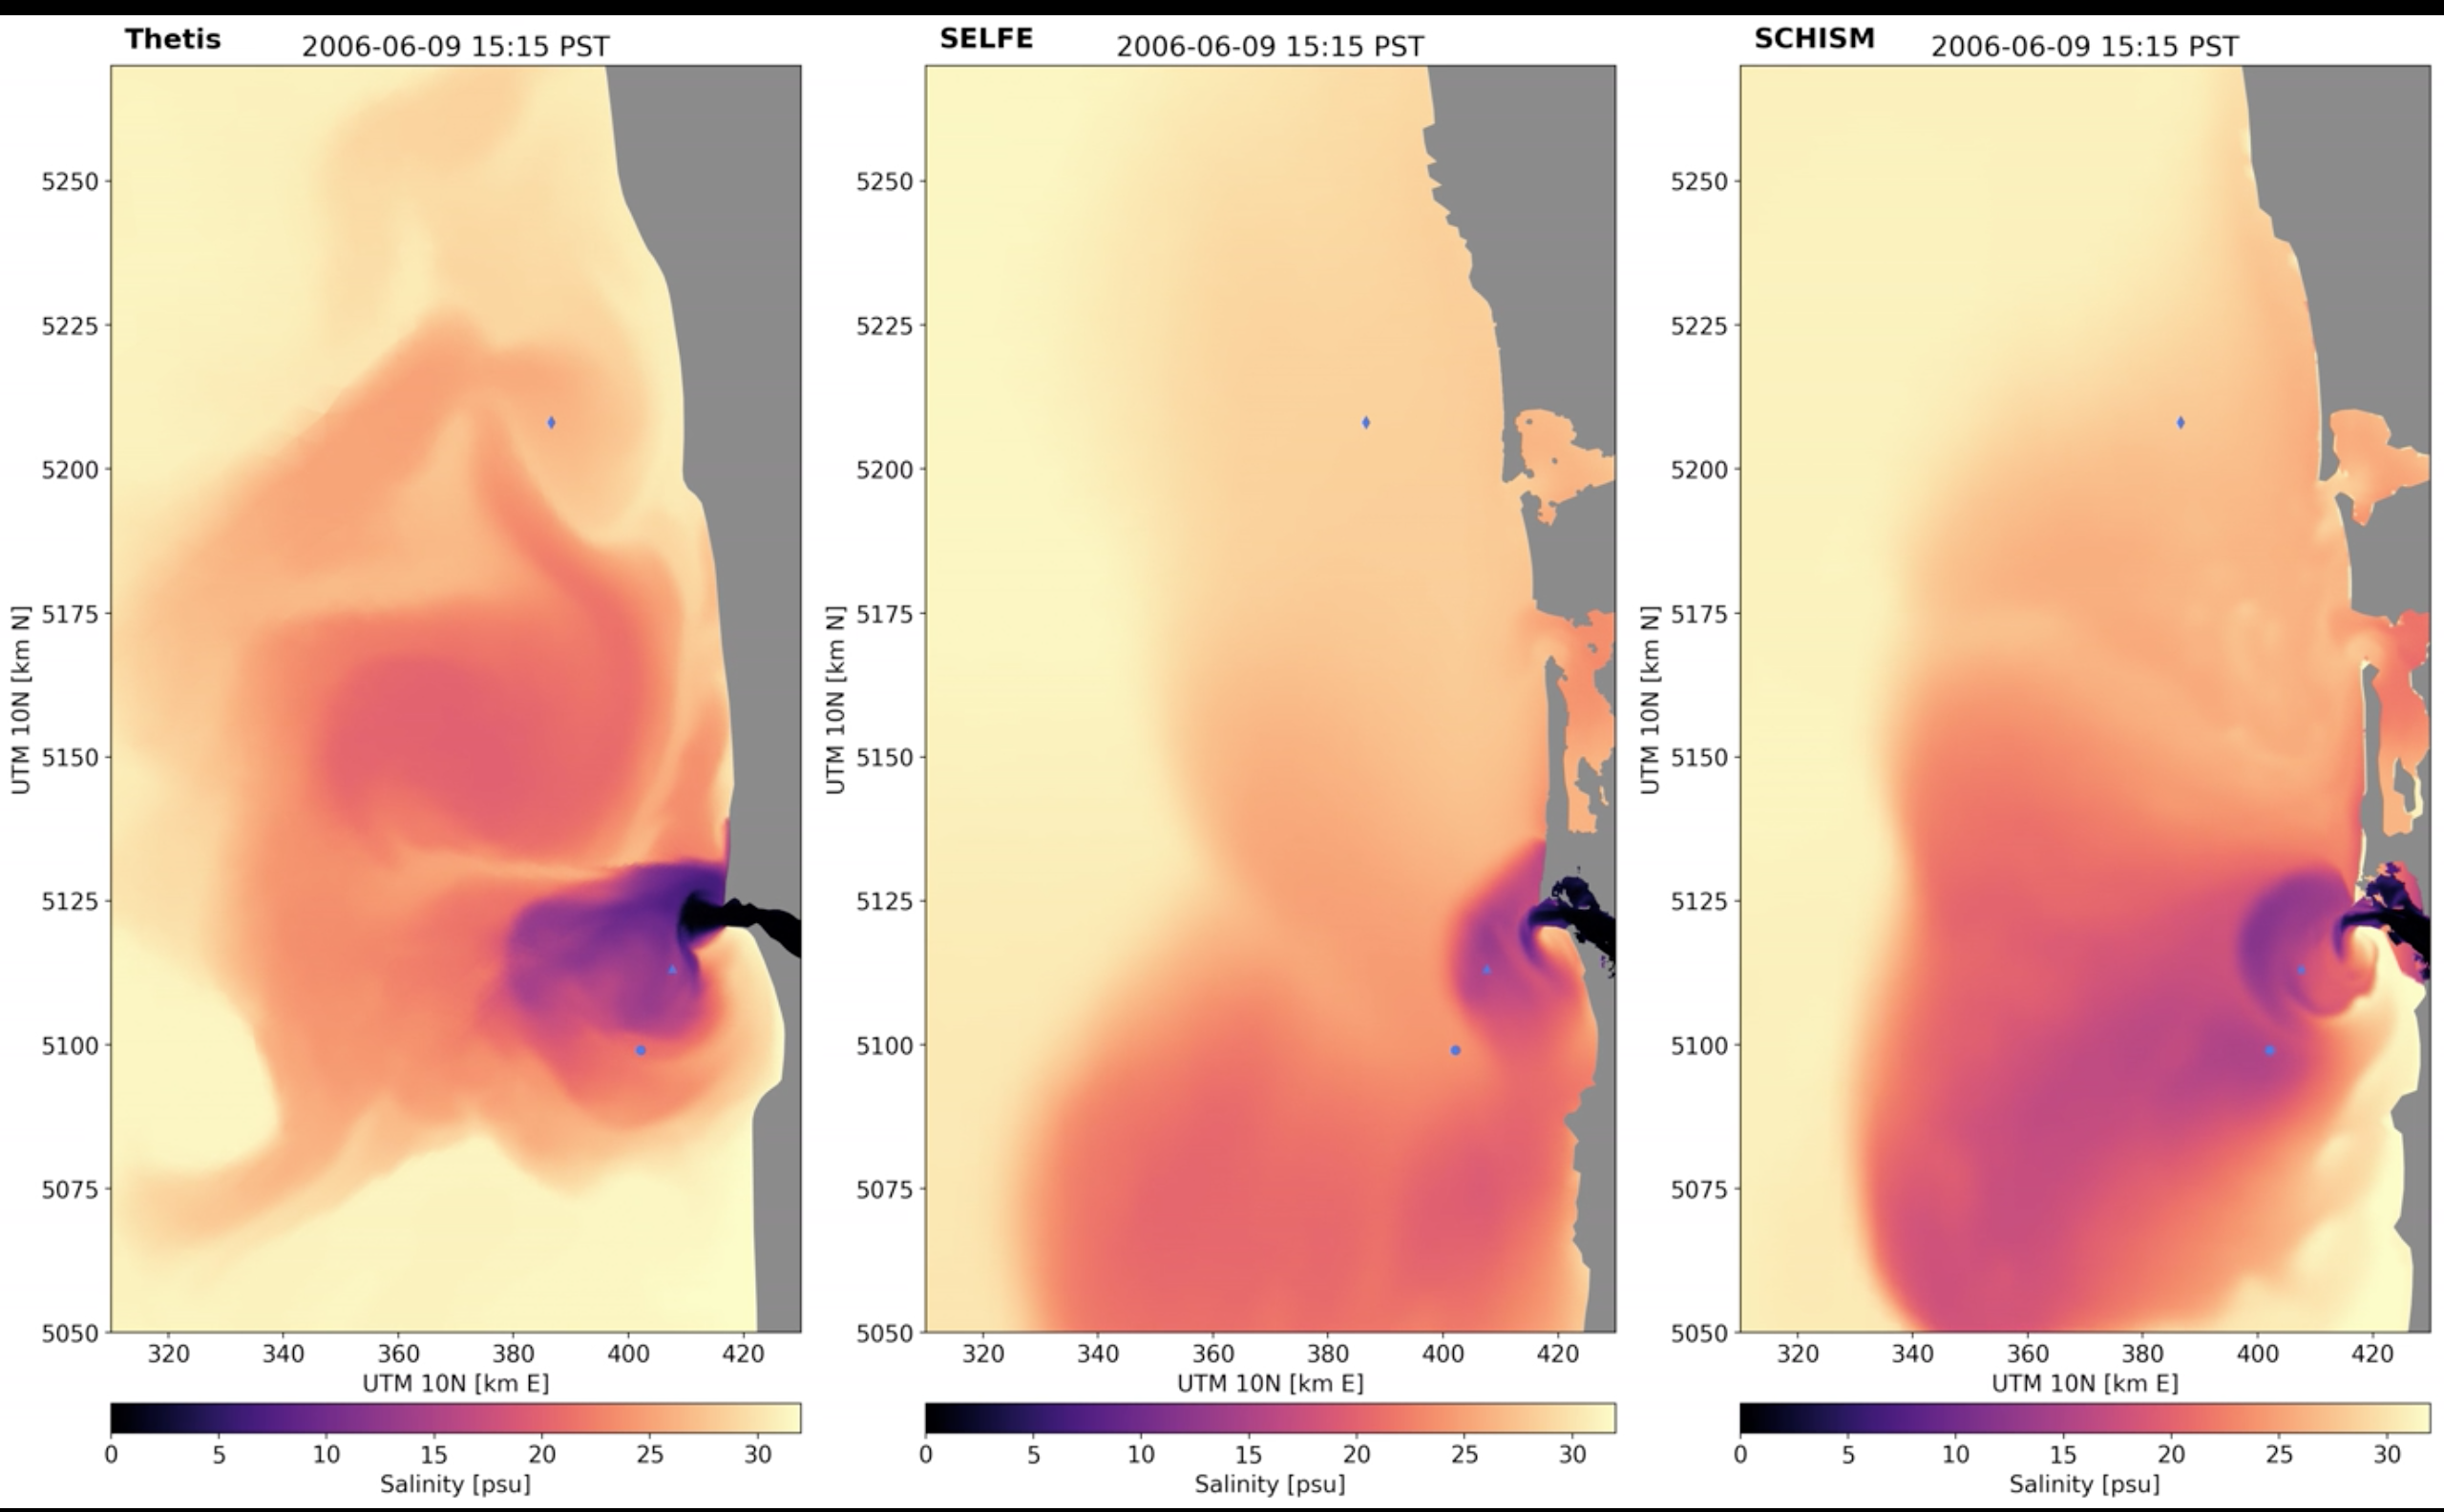
\includegraphics[height=0.45\textheight]{thetis-snapshot}

      {\tiny Surface salinity of the Columbia river plume. Credit
        T.~K\"arn\"a, Finnish Meteorological Institute}

      \url{thetisproject.org}
    \end{column}
    \hspace{-0.04\textwidth}
    \begin{column}{0.48\textwidth}
      \begin{itemize}
      \item Lower numerical mixing, improved results.
      \item 3-8x faster than models with similar quality of results.
      \item Differentiable: efficient adjoint.
      \end{itemize}
      \hfill
\includegraphics[width=1.5cm]{thetis_logo}
    \end{column}
  \end{columns}
  \begin{flushright}
    {\scriptsize T.~K\"arn\"a, S.C.~Kramer, \textbf{LM}, D.A.~Ham, M.D.~Piggott,
    and A.M.~Baptista.  To appear in Geoscientific Model Development, 2018.
    \arxivlink{1711.08552}{physics.ao-ph}\nocite{Karna:2017}}
  \end{flushright}
\end{frame}
\section{Solving sparse systems}

\begin{frame}
  \frametitle{Application challenge}
  \begin{block}{Stationary incompressible Navier-Stokes}
    Find $(u, p) \in \honev \times \ltwo$ such that
    \begin{alignat*}{2}
      -  \nu \nabla^2 u + \advect{u}{u} + \nabla p &= f \quad && \text{ in } \Omega, \label{eqn:momentum} \\
      \nabla \cdot u &= 0 \quad && \text{ in } \Omega, \\
      u &= g \quad && \text{ on } \Gamma_D, \\
      \nu \nabla u \cdot n &= pn \quad && \text{ on } \Gamma_N,
    \end{alignat*}
  \end{block}
  \begin{block}{Discretise and linearise}
    Need to solve linear saddle point system
    \begin{equation*}
      P := \begin{pmatrix}
        A & B^T \\
        B & 0
      \end{pmatrix}
      \begin{pmatrix}
        \delta u \\ \delta p
      \end{pmatrix}
      =
      \begin{pmatrix}
        b \\ 0
      \end{pmatrix}.
    \end{equation*}
  \end{block}
\end{frame}

\begin{frame}
  \frametitle{Challenges for solvers}
  \begin{block}{Desired properties}
    \begin{itemize}
    \item Growth in time to solution is (at worst)
      $\mathcal{O}(n\log n)$.
    \item Convergence does not degree with $\nu \to 0$.
    \end{itemize}
  \end{block}
  \begin{columns}[t]
    \begin{column}{0.5\textwidth}
      \begin{block}{Direct methods}
        \begin{itemize}
        \item[\cmark] Convergence independent of $\nu$
        \item[\xmark] Time to solution $\mathcal{O}(n^2)$ (3D).
        \end{itemize}
      \end{block}
    \end{column}
    \begin{column}{0.5\textwidth}
      \begin{block}{Krylov methods}
        \begin{itemize}
        \item[\cmark] Time to solution $\mathcal{O}(n \log n)$ (with
          multilevel preconditioner)
        \item[\xmark] Convergence independent of $\nu$ challenging
        \end{itemize}
      \end{block}
    \end{column}
  \end{columns}
\end{frame}

\begin{frame}
  \frametitle{Challenges for solvers}
  Want $\nu$- and $h$-independent convergence.
  \begin{block}{Monolithic multigrid: Vanka, Braess-Sarazin smoothing}
    \begin{itemize}
    \item[\cmark] $h$-independent
    \item[\xmark] Convergence degrades with $\nu \to 0$.
    \end{itemize}
  \end{block}
  \begin{block}{Block factorisations}
    \begin{equation*}
      P^{-1} =
      \begin{pmatrix}
        I   & -A^{-1} B^T \\
        0 & I \\
      \end{pmatrix}
      \begin{pmatrix}
        A^{-1}  & 0 \\
        0 & S^{-1} \\
      \end{pmatrix}
      \begin{pmatrix}
        I   & 0 \\
        -BA^{-1} & I \\
      \end{pmatrix}
    \end{equation*}
    Challenges, good approximations to $A^{-1}$ and $S^{-1}$.
  \end{block}
\end{frame}


\begin{frame}
  \frametitle{Block factorisations, approximating $S^{-1}$}
  \only<1>{
    \begin{columns}[t]
      \begin{column}{0.48\textwidth}
        \begin{block}{Pressure mass ($S^{-1} \approx M_p^{-1}$)}
          \begin{itemize}
          \item[\cmark] $h$-independent
          \item[\xmark] Convergence degrades rapidly with $\nu \to 0$
          \end{itemize}
        \end{block}
      \end{column}
      \begin{column}{0.48\textwidth}
        \begin{block}{PCD, LSC ($S^{-1} \approx M_p^{-1} F_p L_p^{-1}$)}
          \begin{itemize}
          \item[\cmark] $h$-independent
          \item[\xmark] Convergence degrades with $\nu \to 0$.
          \end{itemize}
        \end{block}
      \end{column}
    \end{columns}
  }
  \only<2>{
    \begin{block}{Augmented Lagrangian}
      Replace $A \to A + \gamma B^T M_p^{-1}B =: A_\gamma$:
      \begin{equation*}
        P_\gamma := \begin{pmatrix}
          A + \gamma B^T M_p^{-1} B & B^T \\
          B & 0
        \end{pmatrix}
        \begin{pmatrix}
          \delta u \\ \delta p
        \end{pmatrix}
        =
        \begin{pmatrix}
          b \\ 0
        \end{pmatrix}.
      \end{equation*}
      Discrete solution unchanged, since $B\delta u = 0$.

      Then $S^{-1} \approx (\nu + \gamma)M_p^{-1}$ (gets better as
      $\gamma \to \infty$).
      \begin{itemize}
      \item[\cmark] $h$- and $\nu$-independent
      \item[\xmark] $A_\gamma$ is \emph{much} harder to invert than $A$.
      \end{itemize}
      Developed 3D multigrid scheme for $A_\gamma$ extending 2D
      preconditioner of \textcite{Benzi:2006}.
    \end{block}
  }
\end{frame}

\begin{frame}
  \frametitle{A multigrid solver for $A_\gamma$ I: robust smoother}
  $\grad-\div$ term has large kernel: point smoothers not robust.

  \begin{theorem}[Sch\"oberl (1999), Benzi \& Olshanksii (2006)]
    A smoother robust wrt $\nu$ and $\gamma$ requires a subspace
    decomposition
    \begin{equation*}
      V = \sum_i V_i
    \end{equation*}
    such that the kernel is spanned by the subspaces
    \begin{equation*}
      \{u \in V : (\nabla \cdot u, \nabla \cdot v) =
      0 \ \forall\ v \in V\} =: \mathcal{N} = \sum_i \left(V_i \cap \mathcal{N} \right)
    \end{equation*}
  \end{theorem}
\end{frame}

\begin{frame}
  \frametitle{Star smoother}
  \begin{itemize}
  \item Want a \emph{local basis} for the kernel: $\Pzero$ pressure.
  \item Kernel spanned by functions on patch of elements around each
    vertex.
  \item Use overlapping additive Schwarz smoother of ``star'' patches.
  \end{itemize}

  \begin{center}
    \begin{tikzpicture}[scale=4]
      \tikzstyle{v}=[circle, fill, minimum size=0pt, inner sep=0pt]
      \tikzstyle{c}=[diamond, fill, minimum size=4pt, inner sep=0pt]
      \tikzstyle{e}=[rectangle, fill, minimum size=3pt, inner sep=0pt]
      \tikzstyle{select}=[orange, minimum size=5pt]
      \tikzstyle{star}=[magenta]
      \tikzstyle{complete}=[brown]
      \node[v] (v1) at (0, 0) {};
      \node[v] (v2) at (0.25, 0) {};
      \node[v] (v3) at (0.5, 0) {};
      \node[v] (v4) at (0.75, 0) {};
      \node[v] (v5) at (1, 0) {};
      \node[v] (v6) at (0, 0.25) {};
      \node[v] (v7) at (0, 0.5) {};
      \node[v] (v8) at (0, 0.75) {};
      \node[v] (v9) at (0, 1) {};
      \node[v] (v10) at (0.25, 0.25) {};
      \node[v] (v11) at (0.25, 0.5) {};
      \node[v] (v12) at (0.25, 0.75) {};
      \node[v] (v13) at (0.25, 1) {};
      \node[v] (v14) at (0.5, 0.25) {};
      \node[v] (v15) at (0.5, 0.5) {};
      \node[v] (v16) at (0.5, 0.75) {};
      \node[v] (v17) at (0.5, 1) {};
      \node[v] (v18) at (0.75, 0.25) {};
      \node[v] (v19) at (0.75, 0.5) {};
      \node[v] (v20) at (0.75, 0.75) {};
      \node[v] (v21) at (0.75, 1) {};
      \node[v] (v22) at (1, 0.25) {};
      \node[v] (v23) at (1, 0.5) {};
      \node[v] (v24) at (1, 0.75) {};
      \node[v] (v25) at (1, 1) {};

      \draw[thin,gray] (v1) -- (v2) -- (v6) -- (v1);
      \draw[thin,gray] (v2) -- (v10) -- (v6);
      \draw[thin,gray] (v2) -- (v3) -- (v10);
      \draw[thin,gray] (v3) -- (v14) -- (v10);
      \draw[thin,gray] (v3) -- (v4) -- (v14);
      \draw[thin,gray] (v4) -- (v18) -- (v14);
      \draw[thin,gray] (v4) -- (v5) -- (v18);
      \draw[thin,gray] (v5) -- (v22) -- (v18);
      \draw[thin,gray] (v6) -- (v7) -- (v10);
      \draw[thin,gray] (v7) -- (v11) -- (v10);
      \draw[thin,gray] (v11) -- (v14) -- (v15) -- (v11);
      \draw[thin,gray] (v15) -- (v18) -- (v19) -- (v15);
      \draw[thin,gray] (v19) -- (v22) -- (v23) -- (v19);
      \draw[thin,gray] (v7) -- (v8) -- (v11);
      \draw[thin,gray] (v8) -- (v12) -- (v11);
      \draw[thin,gray] (v12) -- (v15) -- (v16) -- (v12);
      \draw[thin,gray] (v16) -- (v19) -- (v20) -- (v16);
      \draw[thin,gray] (v20) -- (v23) -- (v24) -- (v20);
      \draw[thin,gray] (v8) -- (v9) -- (v12);
      \draw[thin,gray] (v9) -- (v13) -- (v12);
      \draw[thin,gray] (v13) -- (v16) -- (v17) -- (v13);
      \draw[thin,gray] (v17) -- (v20) -- (v21) -- (v17);
      \draw[thin,gray] (v21) -- (v24) -- (v25) -- (v21);

      \node[v, select, blue] at (v15) {};
      \node at (barycentric cs:v11=1,v14=1,v15=1) (s1) {};
      \node at (barycentric cs:v14=1,v15=1,v18=1) (s2) {};
      \node at (barycentric cs:v15=1,v18=1,v19=1) (s3) {};
      \node at (barycentric cs:v11=1,v12=1,v15=1) (s4) {};
      \node at (barycentric cs:v12=1,v15=1,v16=1) (s5) {};
      \node at (barycentric cs:v15=1,v16=1,v19=1) (s6) {};
      \draw[thick,blue] \convexpath{s1,s4,s5,s6,s3,s2}{1pt};

      \node[v, select, red] at (v11) {};
      \node at (barycentric cs:v12=1,v11=1,v8=1) (ss1) {};
      \node at (barycentric cs:v7=1,v11=1,v8=1) (ss2){};
      \node at (barycentric cs:v7=1,v10=1,v11=1) (ss3) {};
      \node at (barycentric cs:v14=1,v10=1,v11=1) (ss4) {};
      \draw[thick, red] \convexpath{ss4,ss3,ss2,ss1,s4,s1}{1pt};
    \end{tikzpicture}
  \end{center}
\end{frame}
\begin{frame}
  \frametitle{A multigrid solver for $A_\gamma$ II: robust
    prolongation}

  \begin{theorem}[Sch\"oberl (1999)]
    Let $E_H : V_H \to V_h$, a robust multigrid cycle requires,
    $\forall u_H \in V_H$:
    \begin{equation*}
      \nu \|\nabla(E_H u_H)\|^2_{L^2} + \gamma \|\nabla\cdot (E_H
      u_H)\|^2_{L^2} \le c (\nu \|\nabla(u_H)\|^2_{L^2} + \gamma \|\nabla\cdot u_H\|^2_{L^2})
    \end{equation*}
  \end{theorem}
  Can fix by solving a small Stokes problem for a correction
  in the \emph{interior} of each coarse cell.
    \begin{center}
    \begin{tikzpicture}[scale=4]
      \tikzstyle{v}=[circle, fill, minimum size=0pt, inner sep=0pt]
      \tikzstyle{c}=[diamond, fill, minimum size=4pt, inner sep=0pt]
      \tikzstyle{e}=[rectangle, fill, minimum size=3pt, inner sep=0pt]
      \tikzstyle{select}=[orange, minimum size=5pt]
      \tikzstyle{star}=[magenta]
      \tikzstyle{complete}=[brown]
      \node[v] (v1) at (0, 0) {};
      \node[v] (v2) at (0.25, 0) {};
      \node[v] (v3) at (0.5, 0) {};
      \node[v] (v4) at (0.75, 0) {};
      \node[v] (v5) at (1, 0) {};
      \node[v] (v6) at (0, 0.25) {};
      \node[v] (v7) at (0, 0.5) {};
      \node[v] (v8) at (0, 0.75) {};
      \node[v] (v9) at (0, 1) {};
      \node[v] (v10) at (0.25, 0.25) {};
      \node[v] (v11) at (0.25, 0.5) {};
      \node[v] (v12) at (0.25, 0.75) {};
      \node[v] (v13) at (0.25, 1) {};
      \node[v] (v14) at (0.5, 0.25) {};
      \node[v] (v15) at (0.5, 0.5) {};
      \node[v] (v16) at (0.5, 0.75) {};
      \node[v] (v17) at (0.5, 1) {};
      \node[v] (v18) at (0.75, 0.25) {};
      \node[v] (v19) at (0.75, 0.5) {};
      \node[v] (v20) at (0.75, 0.75) {};
      \node[v] (v21) at (0.75, 1) {};
      \node[v] (v22) at (1, 0.25) {};
      \node[v] (v23) at (1, 0.5) {};
      \node[v] (v24) at (1, 0.75) {};
      \node[v] (v25) at (1, 1) {};

      \draw[thin,gray] (v1) -- (v2) -- (v6) -- (v1);
      \draw[thin,gray] (v2) -- (v10) -- (v6);
      \draw[thin,gray] (v2) -- (v3) -- (v10);
      \draw[thin,gray] (v3) -- (v14) -- (v10);
      \draw[thin,gray] (v3) -- (v4) -- (v14);
      \draw[thin,gray] (v4) -- (v18) -- (v14);
      \draw[thin,gray] (v4) -- (v5) -- (v18);
      \draw[thin,gray] (v5) -- (v22) -- (v18);
      \draw[thin,gray] (v6) -- (v7) -- (v10);
      \draw[thin,gray] (v7) -- (v11) -- (v10);
      \draw[thin,gray] (v11) -- (v14) -- (v15) -- (v11);
      \draw[thin,gray] (v15) -- (v18) -- (v19) -- (v15);
      \draw[thin,gray] (v19) -- (v22) -- (v23) -- (v19);
      \draw[thin,gray] (v7) -- (v8) -- (v11);
      \draw[thin,gray] (v8) -- (v12) -- (v11);
      \draw[thin,gray] (v12) -- (v15) -- (v16) -- (v12);
      \draw[thin,gray] (v16) -- (v19) -- (v20) -- (v16);
      \draw[thin,gray] (v20) -- (v23) -- (v24) -- (v20);
      \draw[thin,gray] (v8) -- (v9) -- (v12);
      \draw[thin,gray] (v9) -- (v13) -- (v12);
      \draw[thin,gray] (v13) -- (v16) -- (v17) -- (v13);
      \draw[thin,gray] (v17) -- (v20) -- (v21) -- (v17);
      \draw[thin,gray] (v21) -- (v24) -- (v25) -- (v21);

      \draw[very thick, black] (v1) -- (v5);
      \draw[very thick, black] (v1) -- (v9);
      \draw[very thick, black] (v3) -- (v17);
      \draw[very thick, black] (v5) -- (v25);
      \draw[very thick, black] (v9) -- (v25);
      \draw[very thick, black] (v7) -- (v23);
      \draw[very thick, black] (v3) -- (v7);
      \draw[very thick, black] (v9) -- (v5);
      \draw[very thick, black] (v17) -- (v23);

      \node[v, select, blue] at (barycentric cs:v7=1,v3=1,v15=1) (cc1) {};
      \node at (barycentric cs:v3=1,v10=1,v14=1) (fc1) {};
      \node at (barycentric cs:v14=1,v15=1,v11=1) (fc2) {};
      \node at (barycentric cs:v7=1,v10=1,v11=1) (fc3) {};
      \draw[thick, blue] \convexpath{fc3,fc2,fc1}{1pt};

      \node[v, select, red] at (barycentric cs:v7=1,v9=1,v15=1) (cc2) {};
      \node at (barycentric cs:v7=1,v8=1,v11=1) (fc4) {};
      \node at (barycentric cs:v8=1,v9=1,v12=1) (fc5) {};
      \node at (barycentric cs:v11=1,v12=1,v15=1) (fc6) {};
      \draw[thick, red] \convexpath{fc4,fc5,fc6}{1pt};
    \end{tikzpicture}
  \end{center}
\end{frame}

\begin{frame}
  \frametitle{3D element pair}
  \begin{columns}
    \begin{column}{0.6\textwidth}
      \begin{block}{Problem}
        $\PtwothreePzero$ is \emph{not} inf-sup for the local Stokes problems.

        $\PthreePzero$ is, but is tremendously expensive for only
        second order convergence in the velocity.
      \end{block}
    \end{column}
    \begin{column}{0.38\textwidth}
      \begin{center}
        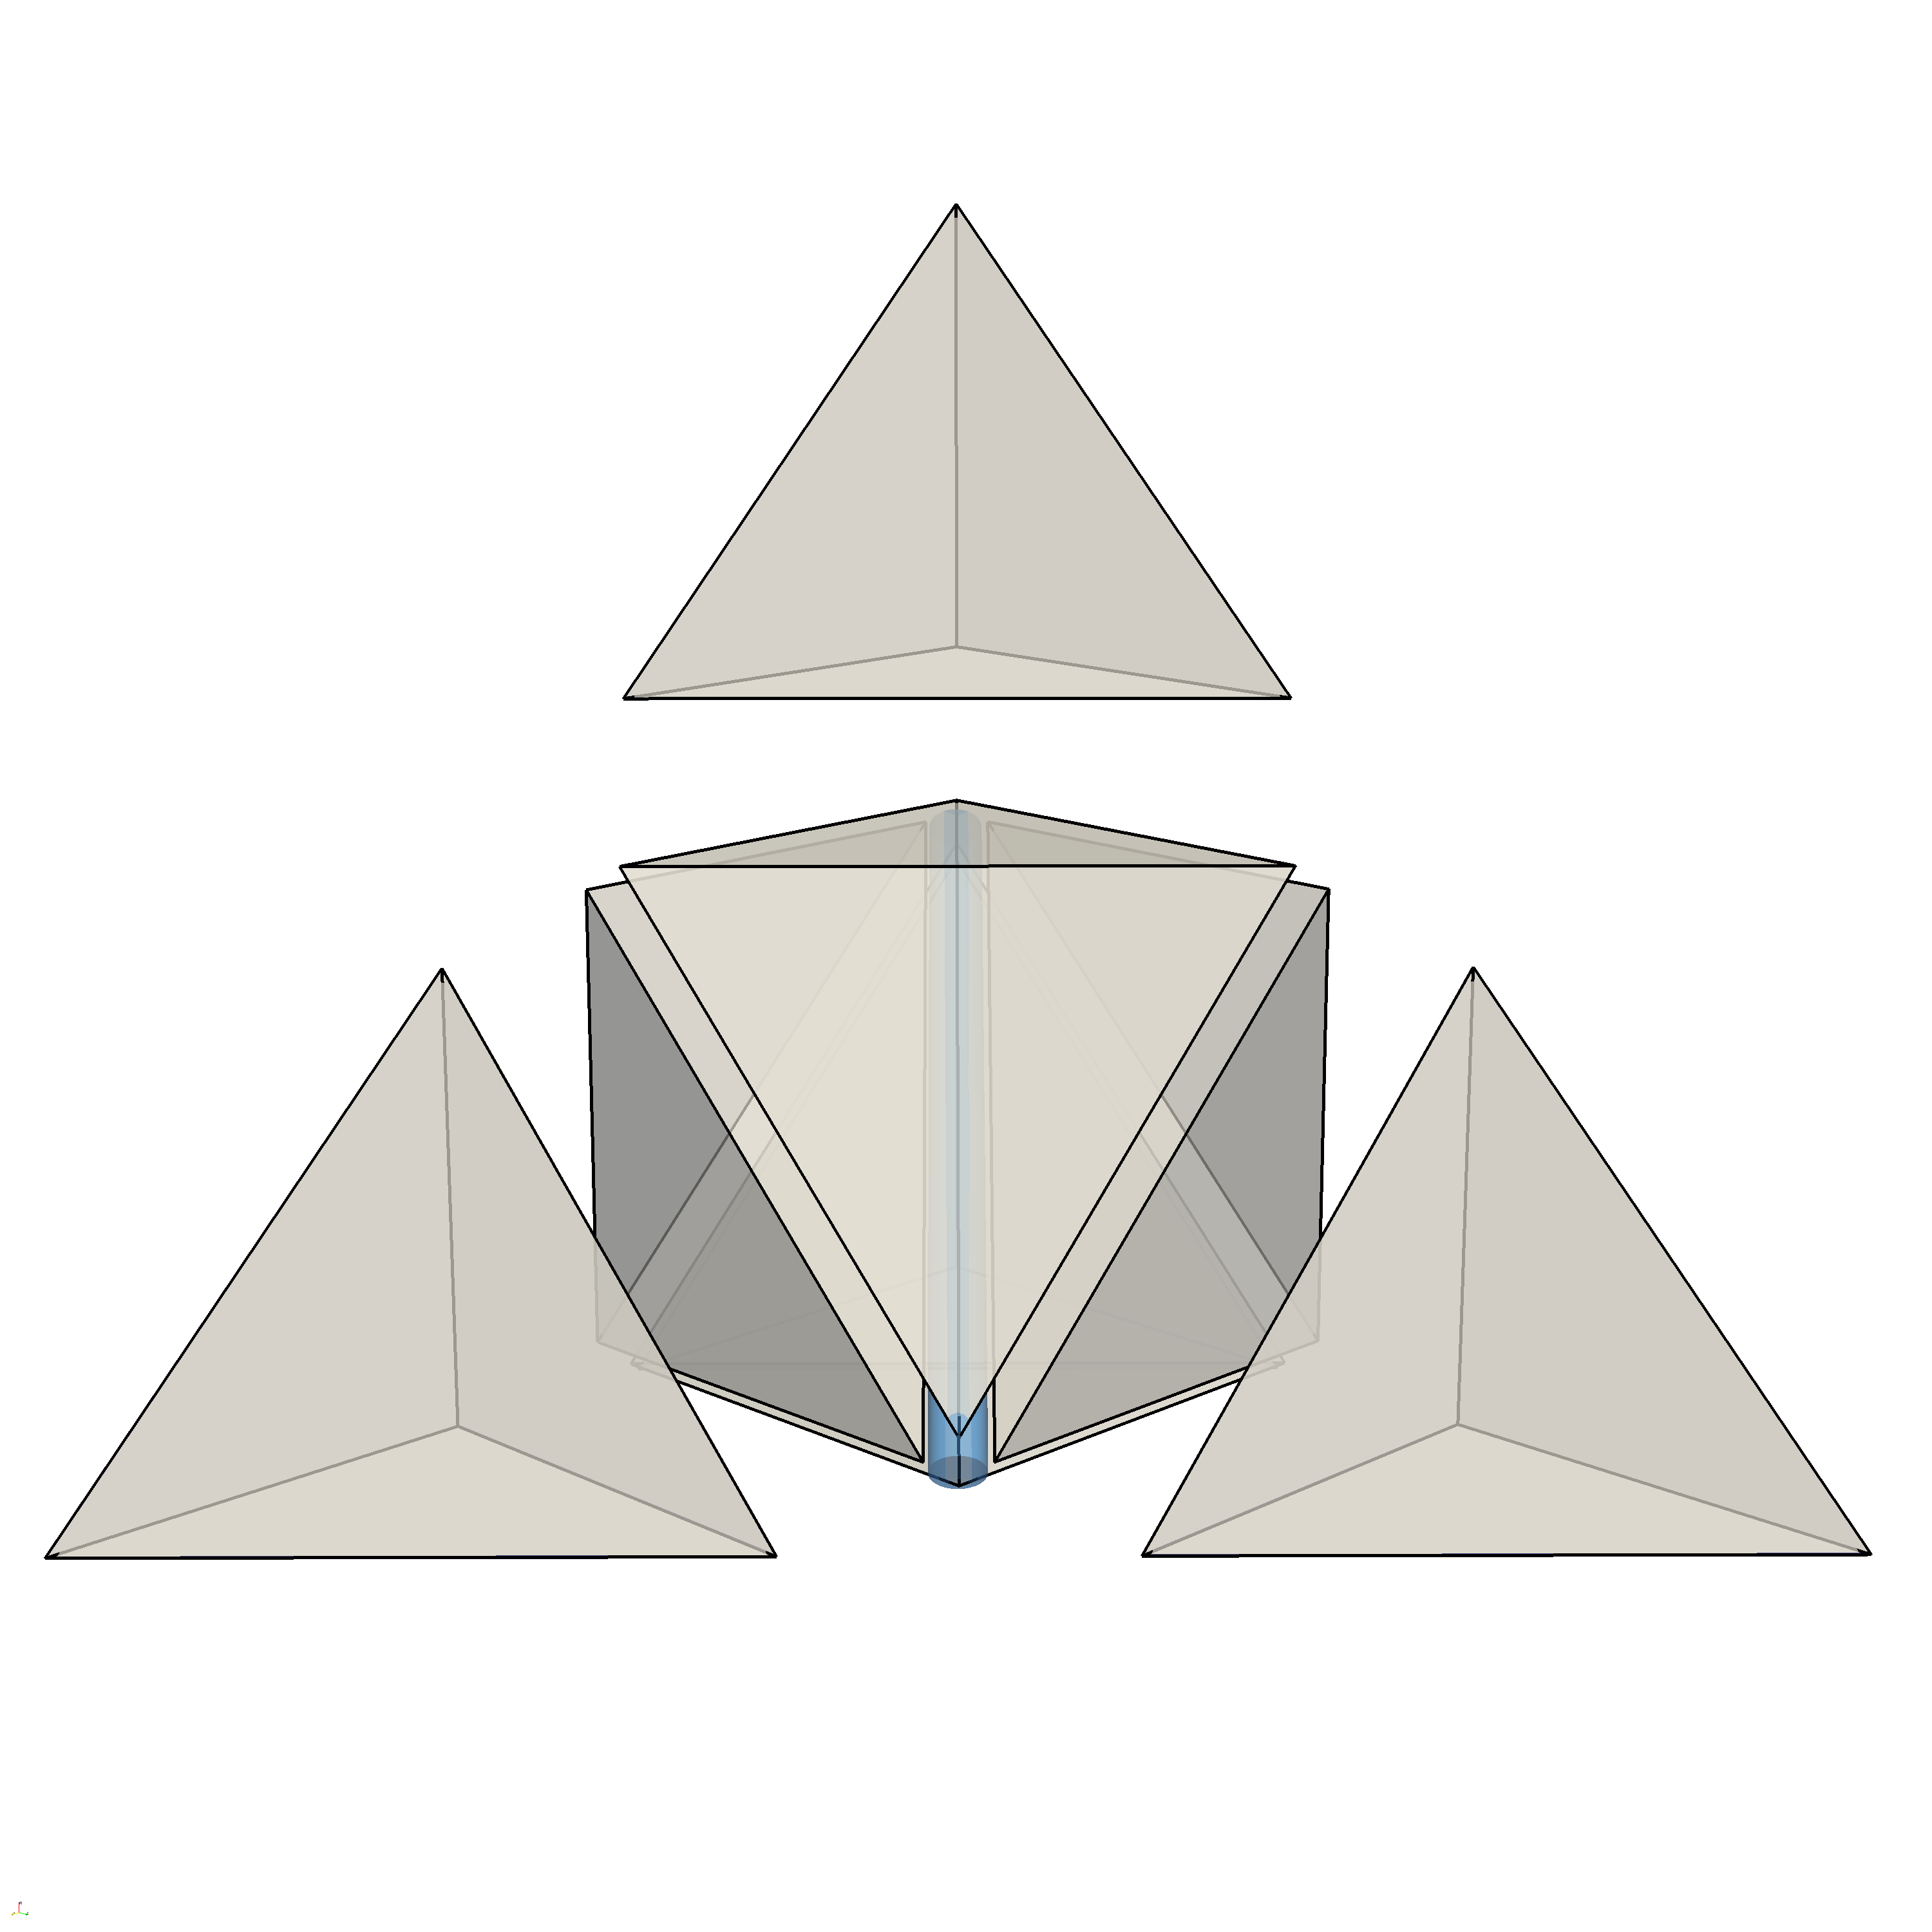
\includegraphics[width=3.5cm]{exploded_tet}
      \end{center}
    \end{column}
  \end{columns}

  \begin{columns}
    \begin{column}{0.6\textwidth}
      \begin{block}{Solution}
        We use an affine-equivalent analog of the Bernardi-Raugel
        element: $\BRzero$.
      \end{block}
    \end{column}
    \begin{column}{0.38\textwidth}
      \begin{center}
        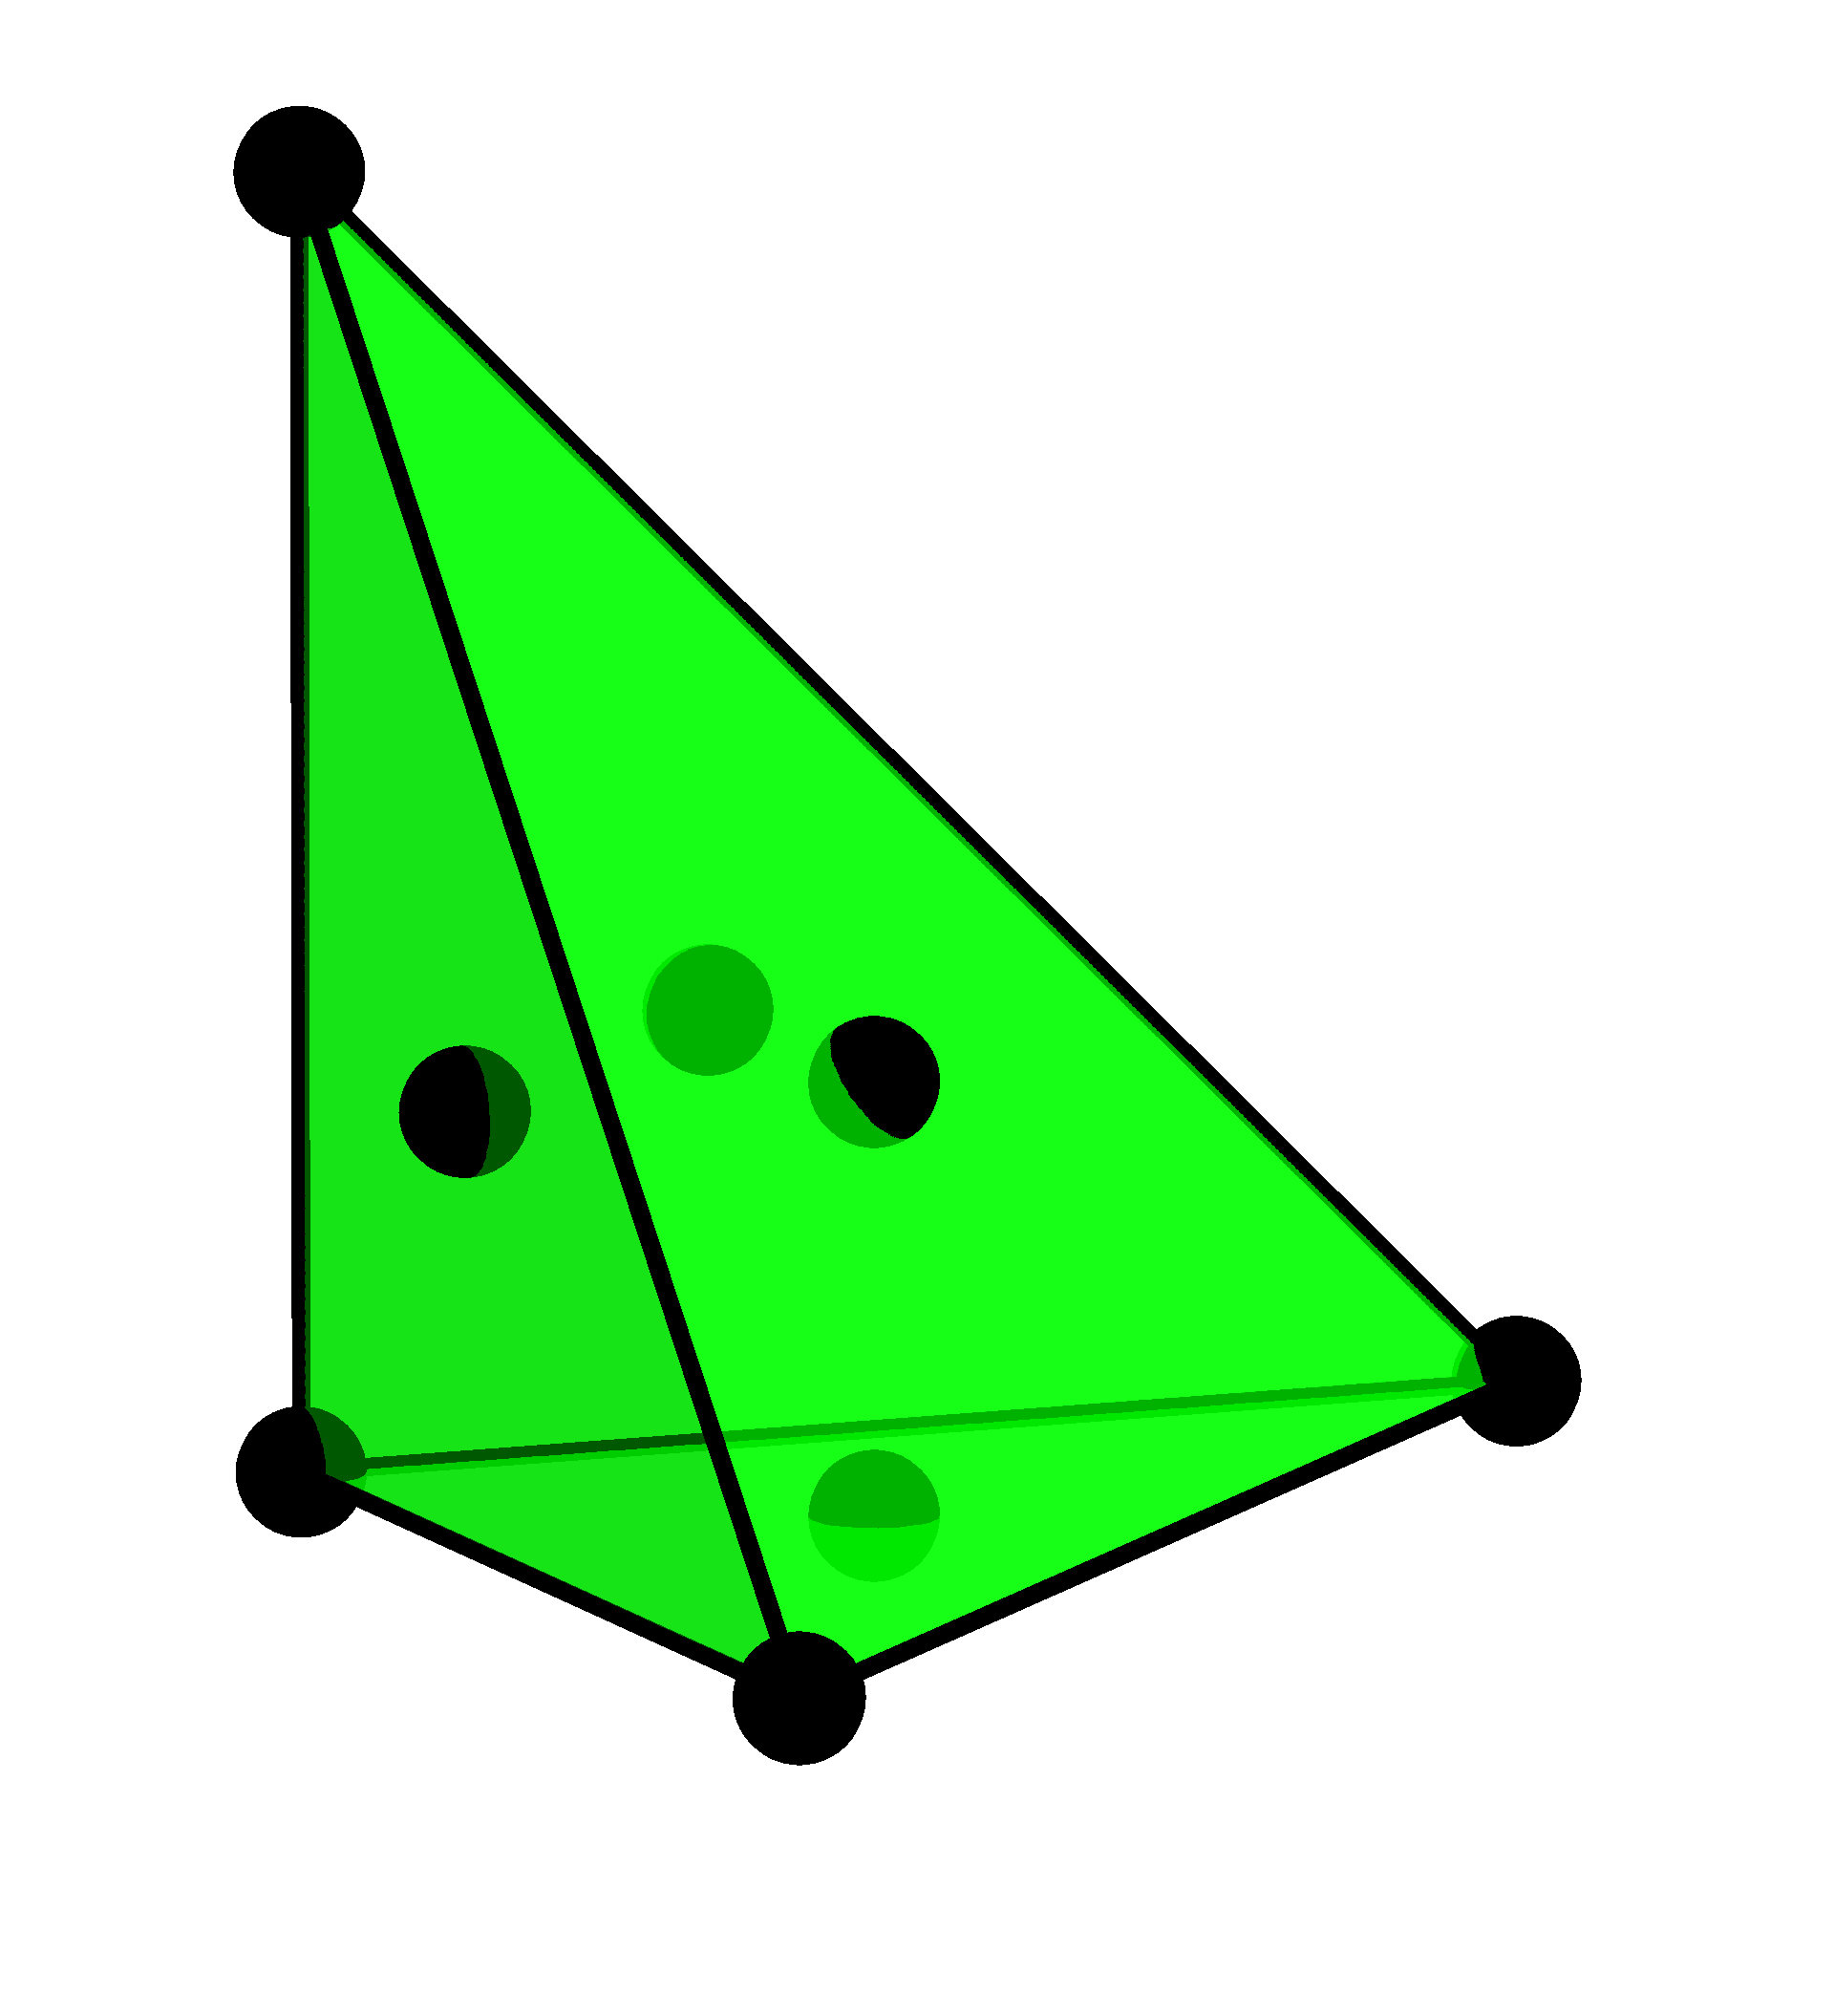
\includegraphics[width=3cm]{P1FB}
      \end{center}
    \end{column}
  \end{columns}
\end{frame}

\begin{frame}
  \frametitle{Preconditioner for flexible additive Schwarz smoothers}
  \begin{itemize}
  \item Solver needs additive Schwarz smoothers in two places.
  \item New in PETSc 3.10 \texttt{-pc\_type patch}
  \end{itemize}
  \begin{block}{Extensible callback interface}
    \begin{itemize}
    \item Separate subspace decompostion (topology + discretisation)
    \item from equation assembly
    \item Extensible mechanism for defining patches
    \item Flexibly supports Vanka, line- and plane-smoothers, \dots
    \item Easy experimentation!
    \end{itemize}
  \end{block}
  \begin{flushright}
    {\scriptsize \textbf{LM}, M.G.~Knepley, P.E.~Farrell, In preparation.}
  \end{flushright}
\end{frame}

\begin{frame}[fragile]
  \frametitle{Multilevel solver}
  \resizebox{\textwidth}{!}{
    \begin{tikzpicture}[
      every node/.style={draw=black, thick, anchor=west},
      grow via three points={one child at (0.0,-0.7) and
        two children at (0.0,-0.7) and (0.0,-1.4)},
      edge from parent path={(\tikzparentnode.210) |- (\tikzchildnode.west)}]
      \node {Continuation}
      child { node {Newton solver with line search}
        child { node {Krylov solver (FGMRES)}
          child { node {Block preconditioner}
            child { node {Approximate Schur complement inverse}}
            child { node {F-cycle on augmented momentum block}
              child { node {Coarse grid solver}
                child { node {LU factorization}}
              }
              child [missing] {}
              child { node {Prolongation operator}
                child { node {Local solves over coarse cells}}
              }
              child [missing] {}
              child { node {Relaxation}
                child { node {GMRES}
                  child { node {Additive star iteration}}
                }
              }
            }
          }
        }
      };
    \end{tikzpicture}
  }
\begin{minted}[fontsize=\tiny]{bash}
$ count-lines .
Language  files  blank  comment  code
Python        4    108      153   558
\end{minted}
\end{frame}

\begin{frame}
  \frametitle{Results: 3D lid-driven cavity}
  \begin{onlyenv}<1>
    \begin{columns}
      \begin{column}{0.48\textwidth}
        \pgfplotstableread[col sep=comma, row sep=\\]{%
          Cores,Time,Dofs\\
          48,1.91e2,2134839\\
          384,2.52e2,16936779\\
          3072,2.3e2,134930451\\
          24576,2.55e2,1077196323\\
        }\datatable
        \begin{tikzpicture}[scale=0.7]
          \begin{semilogxaxis}[
            log basis x=2, ymin=0,
            xtick=data,
            xticklabels from table={\datatable}{Cores},
            extra x ticks={48, 384, 3072, 24576}, extra x tick
            labels={$[2.13]$, $[16.9]$,$[135]$,$[1077]$},
            extra x tick style={tick label style={yshift=-2ex}},
            xlabel={Cores\\{}[DoFs $\times 10^6$]},
            xlabel style={align=center}, ylabel
            near ticks, ylabel style={align=center, text width=4cm},
            ylabel={Time to solution [min]},
            title style={align=center, text width=7cm}]
            \addplot+ table[x=Cores,y=Time] {\datatable};
          \end{semilogxaxis}
        \end{tikzpicture}
      \end{column}
      \hspace{1em}
      \begin{column}{0.48\textwidth}
        \begin{center}
          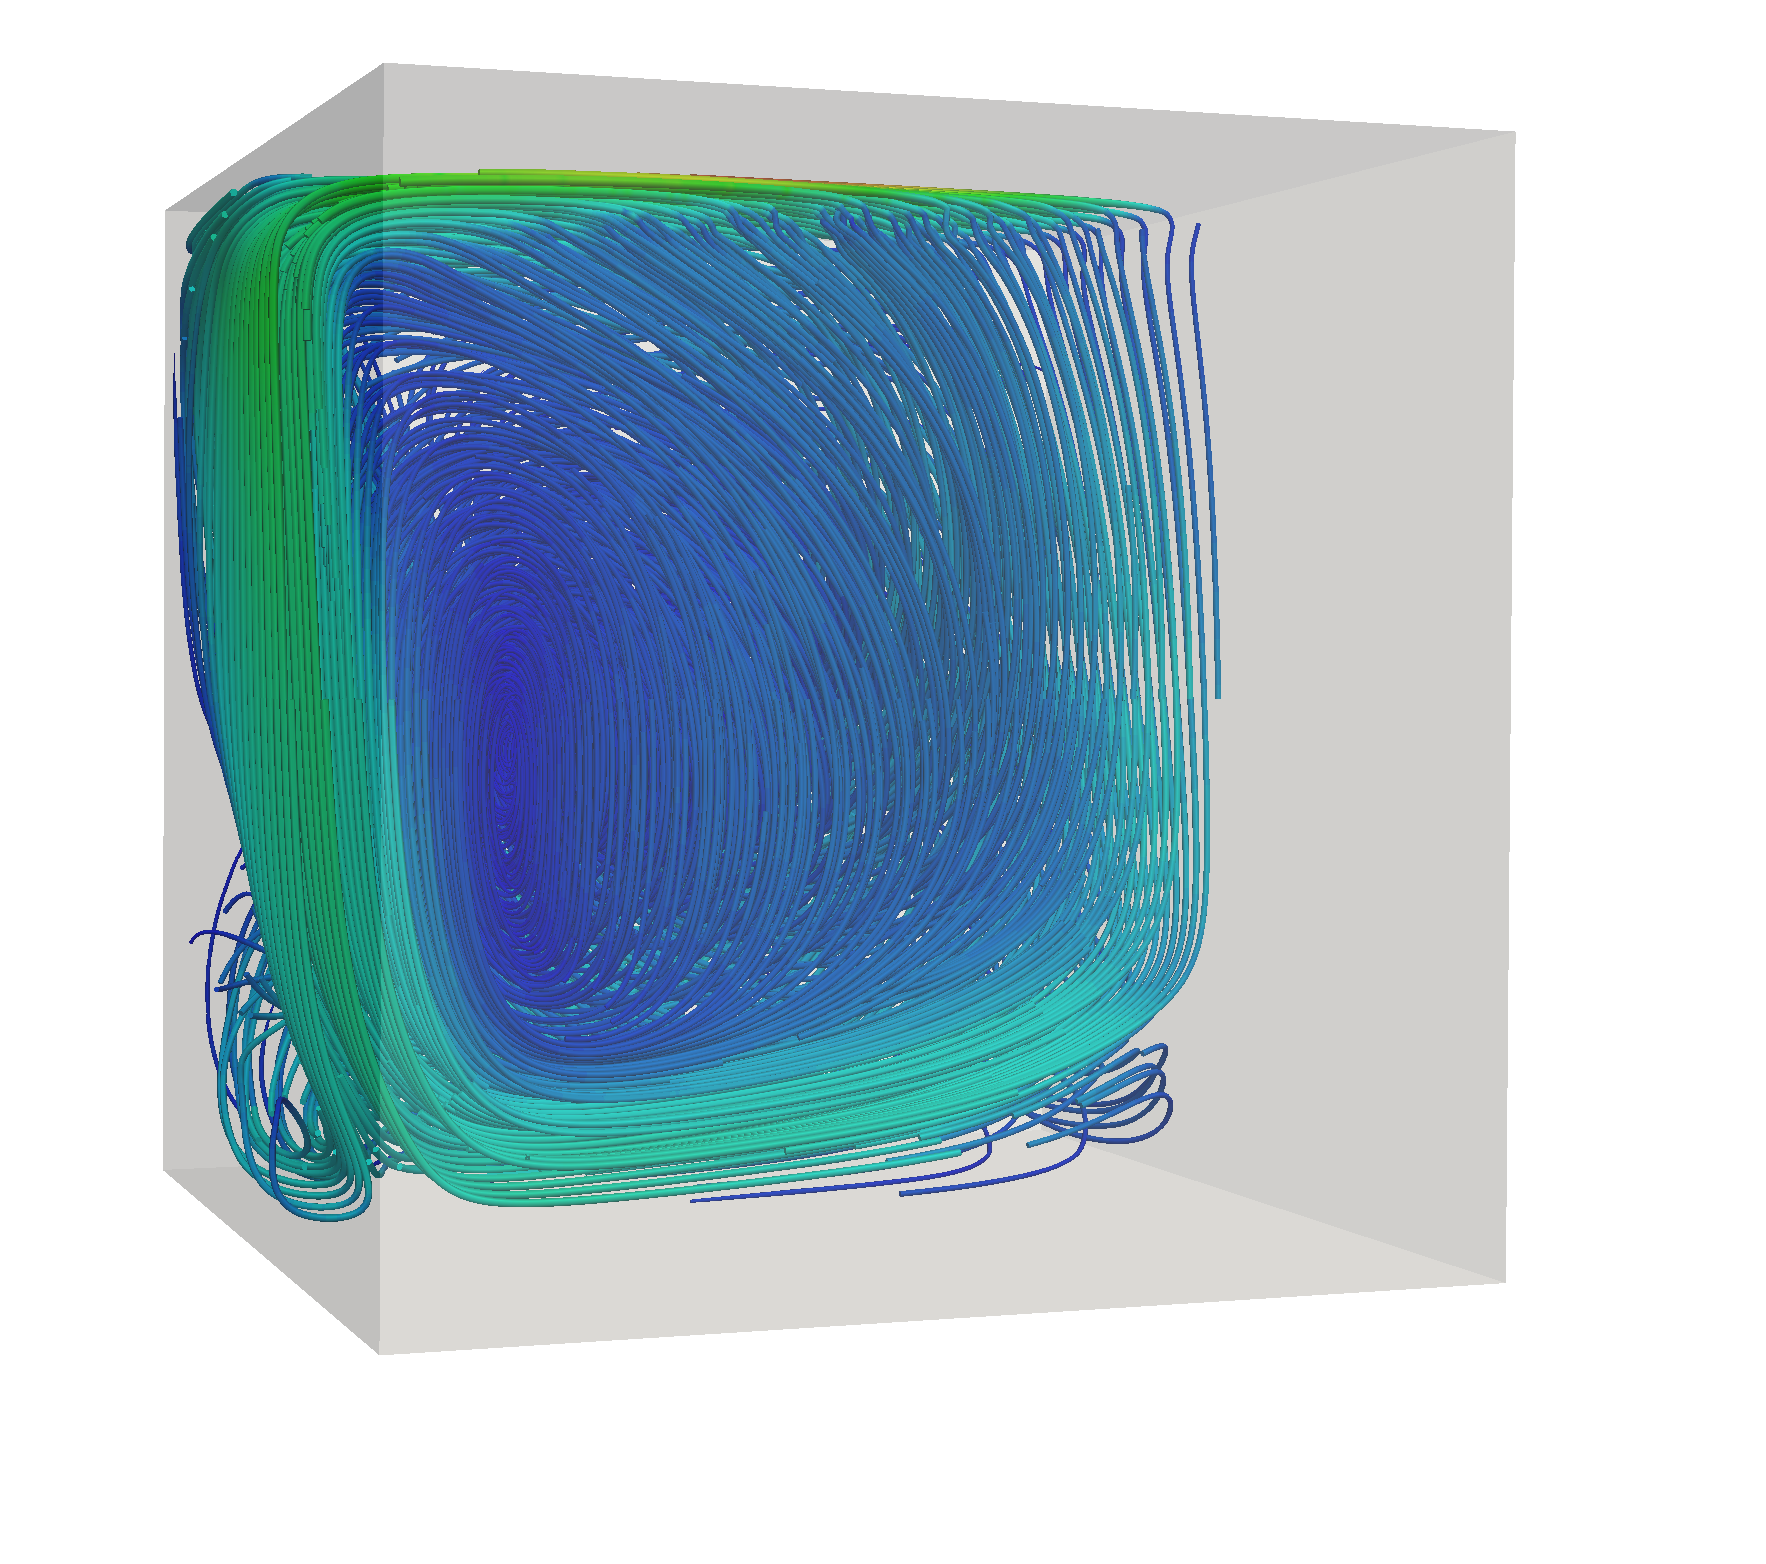
\includegraphics[width=\textwidth]{LDC-streamlines}

          {\tiny Velocity streamlines at Reynolds number 5000.
            Credit F.~Wechsung, University of Oxford.}
        \end{center}
      \end{column}
    \end{columns}
  \end{onlyenv}
  \begin{onlyenv}<2>
    \begin{table}
      \centering
      \begin{tabular}{cc|ccccc}
        \toprule
        \# refinements & \# dofs & \multicolumn{5}{c}{Reynolds number} \\
                       && 10 & 100 & 1000 & 2500 & 5000 \\
        \midrule
        1 & $2.1 \times 10^6$ & 7.50 & 7.33 & 7.50 & 7.00 & 6.50 \\
        2 & $1.7 \times 10^7$ & 8.50 & 7.00 & 7.50 & 6.50 & 5.50 \\
        3 & $1.3 \times 10^8$ & 7.00 & 7.00 & 6.50 & 5.00 & 6.50 \\
        4 & $1.1 \times 10^9$ & 7.00 & 7.33 & 5.50 & 4.00 & 9.00 \\
        \bottomrule
      \end{tabular}
      \caption{Average Krylov iterations per Newton step}
    \end{table}
  \end{onlyenv}
  \begin{flushright}
    {\scriptsize P.E.~Farrell, \textbf{LM}, and F.~Wechsung. In preparation}
  \end{flushright}
\end{frame}

\begin{frame}
  \frametitle{Going forward}
  \begin{itemize}
  \item $\BRzero$ is not a great discretisation
  \item Same ideas should apply to \emph{pressure robust} schemes
    (e.g.~Scott-Vogelius, $H(\div)-L^2$ mixed methods)
  \item Application of same ideas directly to nonlinear multigrid?
  \end{itemize}
  \begin{block}{Idea}
    \begin{itemize}
    \item Preconditioners are formulated in mathematics on paper
    \item They \emph{should} be formulated in mathematics on computer
    \end{itemize}
  \end{block}
\end{frame}
\begin{frame}
  \frametitle{Conclusions \& directions}
  \begin{block}{Automated finite elements}
    \begin{itemize}
    \item Enable significant experimentation
    \item Better code than many humans
    \item Productive mechanism to collaborate with computer science
    \end{itemize}
  \end{block}
  \begin{block}{Fast solvers}
    \begin{itemize}
    \item How to capture mathematical ``building blocks'' in code?
    \item Each class PDE presents different challenges, can we avoid
      doing everything ``from scratch'' each time?
    \end{itemize}
  \end{block}
\end{frame}
\end{document}
